\section{Integrity Policies}

Possiamo distinguere due diversi tipi di integrità:
\begin{itemize}
      \item \textbf{Il livello di integrità di un soggetto} è una misura della
            fiducia che si ripone nella sua
            capacità di produrre o gestire informazioni. Per esempio,
            un'applicazione certificata può
            avere una maggiore integrità rispetto al freeware
            scaricato da internet.
      \item \textbf{Il livello di integrità di un oggetto} descrive il grado
            di “affidabilità” dell'informazione
            contenuta in quell'oggetto.
\end{itemize}

Una meta-policy che i modelli di integrità devono soddisfare è necessariamente
quella di non
permettere che informazioni meno affidabili corrompano quelle più affidabili.
Le informazioni con
bassa integrità non dovrebbero fluire in domini ad alta integrità.
Più alto è il livello, maggiore è la fiducia (trust). Quindi è più probabile
che:
\begin{itemize}
      \item Un programma venga eseguito correttamente;
      \item I dati siano precisi e/o affidabili.
\end{itemize}
\'{E} importante precisare che avere un alto livello di integrità non significa
avere un alto livello di
confidenzialità e viceversa.
In generale se P è un processo con un grado X di “affidabilità”
(\textbf{trustworthiness}) non può
modificare dati ad un livello più alto di lui perché è certificato solo fino
a quel punto; quindi può
modificare o scrivere informazioni nei livelli sottostanti.
I requisiti che una policy di integrità deve rispettare sono:
\begin{itemize}
      \item Gli utenti non possono usare programmi scritti da loro stessi ma
            devono usare programmi e
            DB già esistenti;
      \item Separazione delle funzioni: i programmatori sviluppano e testano
            programmi su un sistema
            diverso da quello di produzione. Quando sono richiesti dei dati in
            fase di testing, non
            vengono presi i dati reali ma dei dati opportunamente modificati
            tramite un processo
            speciale. Tali dati vengono usati solo nella fase di sviluppo e non
            in quella di produzione;
      \item Separazione dei compiti;
      \item Logging and auditing: il processo deve essere controllato,
            verificato (audited), tracciato (logging) e
            deve offrire la possibilità di effettuare un'operazione di rollback;
      \item I manager e coloro che eseguono il processo di verifica devono
            avere accesso ad entrambi
            gli stati dei sistemi ed ai log generati da essi.
\end{itemize}

\subsection{Modello BIBA}

Il modello di integrità Biba venne sviluppato per aggirare le debolezze del
modello di protezione
Bell-LaPadula, il quale non prevedeva la possibilità di eliminazione implicita
degli oggetti di
sicurezza scritti da loro.
Il modello di Biba in generale ha l'obiettivo di preservare l'integrità, ma in
particolare vuole:

\begin{itemize}
      \item Prevenire la modifica dei dati da soggetti non autorizzati;
      \item Prevenire modifiche non autorizzate ai dati da soggetti autorizzati;
      \item Mantenere la consistenza interna ed esterna (es.: dati che
            rispecchino il mondo reale).
\end{itemize}

Implementa le protezioni definendo una serie ordinata di livelli di integrità
per i soggetti e gli
oggetti, rispettando le regole:

\begin{itemize}
      \item \textbf{Read Up:} Questo significa che
            un soggetto che si trova al livello di integrità X può leggere
            solo oggetti allo stesso livello o
            superiore (“assioma di integrità semplice”);
      \item \textbf{Write Down:} un soggetto al livello di integrità X può
            scrivere solo oggetti allo stesso livello
            o di livello più basso (assioma di integrità * o Proprietà di
            semplice sicurezza);
\end{itemize}
Un esempio è quello della gerarchia militare: un generale può solo ricevere
ordini dai suoi superiori o parigrado e può imporre ordini solo ai suoi
sottoposti o parigrado per evitare un cambiamento/danneggiamento
nella missione da svolgere.
Da notare che \textit{Read Up} e \textit{Wite Down} sono l'opposto delle regole
\textit{Read Down}, \textit{Write Up} del modello Bell-LaPadula.\\

È impossibile trasformare informazioni meno trusted in più trusted.
L'obiettivo di tale modello è quello di evitare che il grado di fiducia di
un'informazione aumenti. Se ciò
si verificasse, si potrebbe considerare fidata un'informazione che in realtà
non lo è.
Ad ogni risorsa del sistema viene assegnata un'\textit{etichetta} indicante
il livello di integrità minimo
richiesto per l'accesso da parte dei soggetti. Le etichette di integrità,
non coincidono con quelle di
confidenzialità: le prime limitano le modifiche che si possono fare alle
informazioni, mentre le
seconde limitano il flusso delle informazioni. Maggiore è il livello di
integrità e maggiore è la
certezza che un programma sia eseguito correttamente e che i dati siano accurati
e veritieri.
Esistono delle relazioni tra integrità e la sua affidabilità. I livelli di
integrità sono un punto
importante per la sicurezza ma non coincidono con i livelli di sicurezza.\\

Ricordarsi che i modelli Bell-LaPadula e BIBA sono in conflitto tra loro e
non si possono utilizzare
contemporaneamente.

\subsection{Modello Clark-Wilson}

Rappresenta un'alternativa al modello di Biba ed utilizza le transazioni come
operazioni base per
garantire integrità prima e dopo le operazioni.
Si basa su questi tre principi:

\begin{itemize}
      \item \textbf{Separazione dei compiti}: Se sono necessarie due o più fasi per
            eseguire una funzione,
            almeno due persone devono eseguire le fasi separandosi adeguatamente
            i compiti;
      \item \textbf{Separazione delle funzioni}:
            \begin{itemize}
                  \item Una singola persona non può svolgere ruoli complementari
                        in un processo critico;
                  \item Gli sviluppatori non sviluppano nuovi programmi sui
                        sistemi di produzione;
                  \item Gli sviluppatori non elaborano i dati di produzione sui
                        sistemi di produzione;
            \end{itemize}
      \item \textbf{Auditing}: I sistemi commerciali sottolineano l'importanza del
            recupero e della responsabilità
            (recoverability e accountability). I sistemi vengono analizzati per
            determinare quali azioni
            hanno avuto luogo e chi è stato coinvolto.
\end{itemize}

In generale un dato si può trovare in uno stato consistente o non consistente,
in particolare si
troverà nello stato consistente o valido se soddisfa un insieme di vincoli
(definizione di integrità
secondo Clark Wilson).
I tasselli alla base del modello CW sono quindi:

\begin{itemize}
      \item \textbf{Autenticazione}: l'identità di tutti gli utenti deve essere
            autenticata correttamente;
      \item \textbf{Audit}: le modifiche devono essere tracciate (logging) per registrare ogni
            programma eseguito e da chi,
            in modo che non possa essere annullato;
      \item \textbf{Transazioni ben formate}: gli utenti manipolano i dati solo in modo
            limitato. Sono consentiti
            solo accessi legittimi;
      \item \textbf{Separazione dei compiti}: il sistema associa ad ogni utente un
            insieme di programmi che
            può eseguire. Impedisce le modifiche non autorizzate, preservando
            così l'integrità;
\end{itemize}

\paragraph{Esempio.}\ \\

\begin{figure}[H]
      \centering
      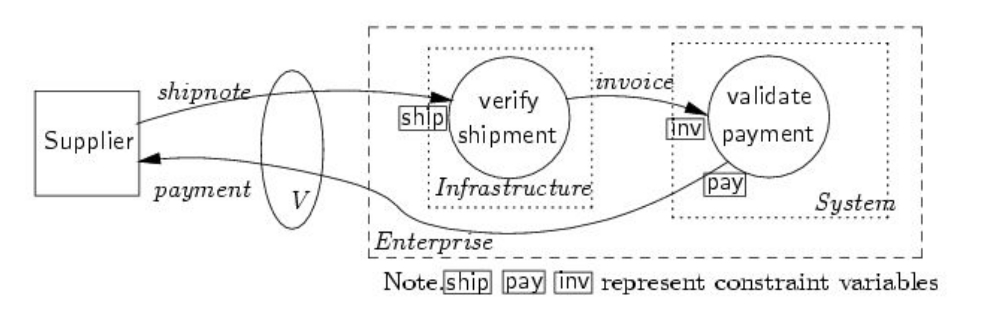
\includegraphics[width=\textwidth, keepaspectratio]{capitoli/policy/imgs/clark_wilson.png}
\end{figure}

Consideriamo il momento in cui il fornitore consegna la merce ad una specifica e
ciò è testimoniato dalla shipnote, ovvero la bolla di consegna. Una possibile
organizzazione dell'impresa prevede che vi sia una persona addetta al magazzino
che verifica se la merce ricevuta corrisponde a quella specificata nella bolla.
Se così è, viene generata la fattura e avviene il pagamento per la merce. Un
vincolo di integrità che vogliamo avere (dal lato dell'azienda) è che venga
pagato solo quello che è stato consegnato, quindi che il valore del pagamento
sia minore o uguale a quello indicato nella bolla di consegna. Il discorso è
inverso per il lato del fornitore.\\

C'è poi una \textit{Seconda Organizzazione} in cui la bolla viene affidata a due
persone (separazione dei compiti): entrambe verificano che ciò che è stato
consegnato corrisponda a quanto indicato dalla bolla ed eventualmente la
inoltrano all'ufficio pagamenti. L'ufficio deve a questo punto constatare che le
due comunicazioni siano coerenti tra loro.

\begin{figure}[H]
      \centering
      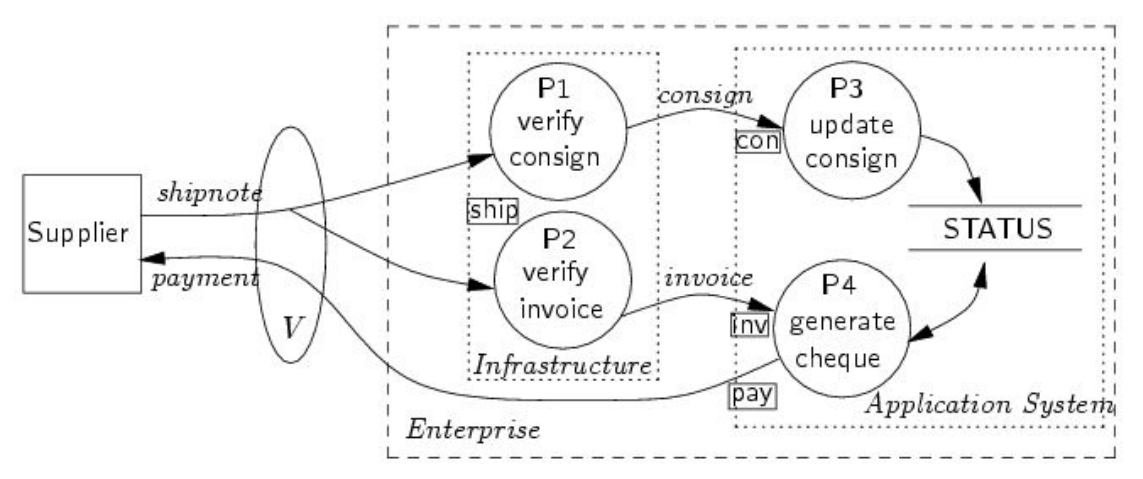
\includegraphics[width=\textwidth, keepaspectratio]{capitoli/policy/imgs/clark_wilson2.png}
\end{figure}

Questo secondo sistema è più forte e ciò può essere verificato formalmente:
\begin{itemize}
      \item funziona lo stesso anche se interviene un utente disonesto;
      \item può essere attaccato, ma occorrono due operai disonesti che scrivono
            bolle con importi più alti rispetto al valore reale;
      \item se un attacco dovesse avere successo, il sistema non risulta essere
            più sicuro dal lato integrità.
\end{itemize}

\subsubsection{Come funziona?}

Il modello Clark-Wilson è di tipo MAC e le regole sono decise dal sistema e non
dagli utenti.
Si basa su altri due concetti chiave:

\begin{itemize}
      \item Una transazione deve essere ben formata (WFT), cioè deve far passare
            il sistema da uno
            stato consistente verso altri stati consistenti. E' pertanto
            importante stabilire un
            meccanismo che permetta di esaminare e certificare che le transazioni
            siano eseguite
            correttamente;
      \item Viene rispettato il principio della separazione dei compiti:
            l'operazione viene divisa in
            sottoparti che devono essere eseguite da soggetti differenti.
            In questo modo, per attuare
            una frode, ad esempio, è necessario che tutti i soggetti delle
            transazioni ne siano
            consapevoli. In pratica vi è una distinzione tra colui che esegue
            una transazione e colui che
            la certifica.
\end{itemize}

Il modello di Clark-Wilson richiede che il Sistema Informativo, nel quale viene
applicato, disponga
delle seguenti caratteristiche essenziali:

\begin{itemize}
      \item Autenticazione da parte degli utenti;
      \item I dati possono essere manipolati da uno specifico set di procedure,
            che a loro volta
            possono essere eseguite solo da un utente autorizzato;
      \item Vengono mantenuti i log (contenenti programmi, dati e nomi degli
            utenti);
      \item I meccanismi di protezione non possono essere cambiati (staticità);
      \item Il security officer è il responsabile degli assegnamenti;
      \item Specifiche regole di sicurezza per la modifica dei dati.
\end{itemize}

\begin{figure}[H]
      \centering
      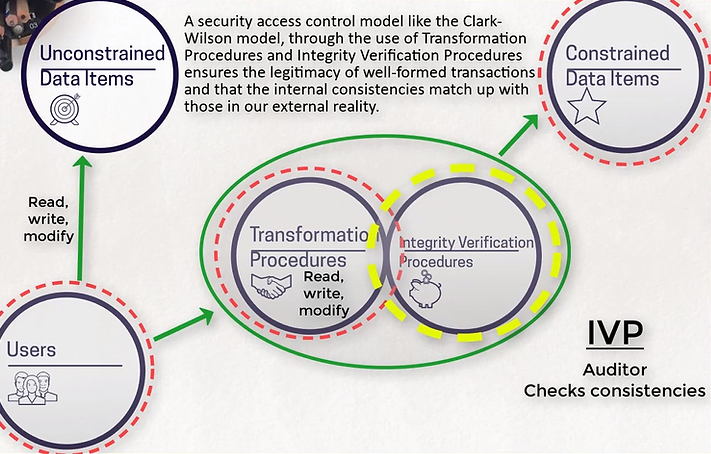
\includegraphics[width=12cm, keepaspectratio]{capitoli/policy/imgs/clark_wilson3.png}
\end{figure}

Formalmente il modello suddivide i dati in due set:

\begin{itemize}
      \item \textbf{CDI} (\textit{Constrained Data Item}): contiene gli elementi
            del sistema da proteggere, ossia i dati
            soggetti al controllo di integrità. Ad esempio in una banca, il CDI
            potrebbe essere composto
            dal saldo dei conti;
      \item \textbf{UDI} (\textit{Unconstrained Data Item}): contiene l'insieme
            dei dati non soggetti ai vincoli di
            integrità.
\end{itemize}

L'appartenenza dei dati ad una determinata classe è esclusiva.
Il modello prevede due tipi di procedure:

\begin{itemize}
      \item \textbf{IVP} (\textit{Integrity Verification Procedures}): è
            l'insieme delle funzioni che verificano se un
            determinato set di dati, appartenenti alla classe CDI, soddisfa
            determinati vincoli di
            integrità, i quali sono implementati come vincoli nel linguaggio SQL;
      \item \textbf{TP} (\textit{Transformation Procedures}): è l'insieme delle
            procedure di trasformazione che hanno in input
            ed in output dei dati appartenenti alla classe CDI. Se un set dati
            CDI di partenza soddisfa
            un determinato IVP, allora lo soddisferà anche il set CDI ottenuto
            dopo la trasformazione;
            questo risulterà vero solo se la procedura è ben formata.
\end{itemize}

Le procedure tipo IVP permettono di garantire che il sistema parta da uno stato
consistente,
mentre le procedure TP assicurano che lo stato sarà consistente anche in futuro.
Una tipica
transazione nel database è composta da TP, le quali trasformano dati UDI in CDI
oppure
aggiornano dati CDI.
Una IVP quindi garantisce che tutti i CDI nel sistema siano validi in un
determinato stato. Un TP,
invece, prende in input un CDI o un UDI e produce sempre un CDI.
Il modello utilizza le transazioni come operazioni di base. L'integrità deve
essere garantita prima e
dopo le operazioni; di conseguenza i dati possono trovarsi in uno stato coerente
oppure
inconsistente. L'integrità viene definita mediante vincoli che i dati devono
rispettare.
Definire le caratteristiche di una transazione ben formata è un lavoro manuale
eseguito da un
security officer, il quale è l'unico che può specificare il set di procedure che
possono modificare
certi CDI.

\begin{figure}[H]
      \centering
      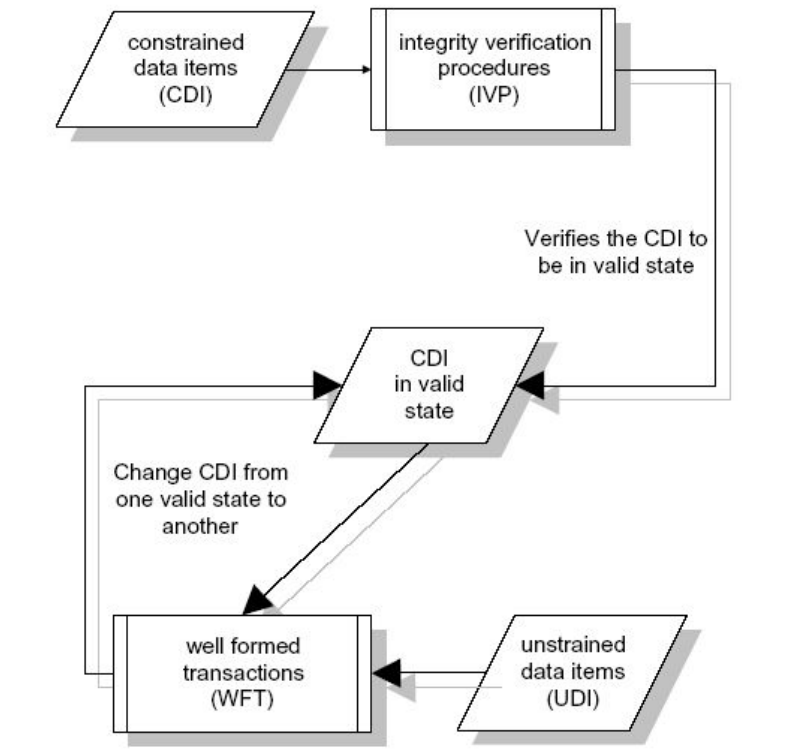
\includegraphics[width=8cm, keepaspectratio]{capitoli/policy/imgs/clark_wilson4.png}
\end{figure}

Nel caso debbano entrare nel sistema degli UDI questi devono essere processati
solo da WFT per
risultare CDI.
Il minimo di sicurezza richiesta comprende:
\begin{itemize}
      \item Integrità: i vincoli d'integrità esistono per proteggere IS da
            maligni o accidentali modifiche
            dei dati. Le regole possono essere definite su stati statici del db
            o su transazioni (es. prima
            di poter effettuare un modifica);
      \item Identificazione, autenticazione: prima di accedere a un sistema ogni
            utente deve essere
            identificato e autenticato per mantenerne traccia e per dargli
            l'accesso;
      \item Autorizzazioni (cioè controllo sugli accessi)
\end{itemize}

\subsubsection{Regole di certificazione}
Al fine di garantire la validità dei dati nel sistema, il modello di
Clark-Wilson prevede le seguenti
regole di certificazione:
\begin{itemize}
      \item \textbf{CR1} se un IVP è eseguito, deve assicurarsi che tutti i CDI
            siano in uno stato valido.
      \item \textbf{CR2} una TP deve trasformare un insieme di CDI da uno stato
            valido ad uno valido
            \begin{itemize}
                  \item CR2 definisce come “certificata” una relazione che
                        associa un insieme di CDI ad
                        una TP;
                  \item CR2 implica che una TP può corrompere una CDI se non è
                        certificata per lavorare
                        con quel CDI
                        \begin{itemize}
                              \item \textit{Esempio}: la TP che investe denaro nel
                                    portafoglio azionario della banca
                                    corromperebbe i bilanci anche se la TP
                                    fosse certificata a lavorare sul
                                    portafoglio, poiché le azioni della TP
                                    potrebbero non avere senso sui conti
                                    bancari
                              \item Da ciò nasce la prima regola di rinforzo
                        \end{itemize}
            \end{itemize}
\end{itemize}

\subsubsection{Regole di rinforzo}

Tutte le TP devono essere certificate per essere valide.
Un TP può manipolare in modo errato (cioè non conforme ad un IVP) un CDI se
non è stato
certificato a lavorare per questo. Per evitare il problema, esistono delle
regole di rinforzo
(enforcement):

\begin{itemize}
      \item \textbf{ER1} Il sistema deve garantire che solo le TP certificate ad
            operare su determinati CDI svolgano
            operazioni su di essi.
      \item \textbf{ER2} Il sistema deve associare a ciascun TP un utente e un
            insieme di CDI su cui l'utente e la TP possono lavorare. Il TP può
            accedere a quei CDI per conto dell'utente, ma non può accedere per conto di
            utenti non autorizzati.
            \begin{itemize}
                  \item Il sistema deve mantenere le relazioni certificate;
                  \item Il sistema deve restringere l'accesso degli utenti alle
                        TP mediante una relazione di
                        permesso che specifica quali utenti possono eseguire
                        certi TP e su quali CDI.
            \end{itemize}
\end{itemize}

\subsubsection{Utenti e regole}

\begin{itemize}
      \item \textbf{CR3} Le relazioni di permesso devono essere basate sulla
            separazione dei compiti.
      \item \textbf{ER3} Il sistema deve autenticare ogni utente che vuole
            utilizzare una TP.
\end{itemize}

\subsubsection{Uso dei Log}

\begin{itemize}
      \item \textbf{C4} Tutte le TP devono scrivere in CDI di solo accodamento
            (append) tutte le informazioni
            sufficienti a ricostruire le operazioni svolte.
            \begin{itemize}
                  \item Questo CDI è il log;
                  \item Gli amministratori devono essere in grado di capire
                        cosa ha fatto una determinata
                        transazione.
            \end{itemize}
\end{itemize}

\subsubsection{Trattamento di input non fidato}

\begin{itemize}
      \item \textbf{CR5} Ogni TP che prende in input un UDI può eseguire solo
            trasformazioni valide, oppure
            nessuna trasformazione, per ogni possibile valore dell'UDI.
            La trasformazione può quindi rifiutare il
            UDI o trasformarlo in un CDI.
            \begin{itemize}
                  \item Un possibile esempio: in un banca i numeri inseriti
                        da tastiera sono UDI, i quali non possono essere dati in input
                        ad una TP. Un'apposita TP deve validare tali numeri
                        (rendendoli un CDI) prima di usarli; se
                        la validazione fallisce, la TP rigetta il UDI.
            \end{itemize}
\end{itemize}

\subsubsection{Separazione dei compiti}

\begin{itemize}
      \item \textbf{ER4} Solo il certificatore di un TP può cambiare la lista di
            entità associate al TP. Nessun
            certificatore di un TP, o di un'entità associata al TP, potranno mai
            farlo.
\end{itemize}

\begin{figure}[H]
      \centering
      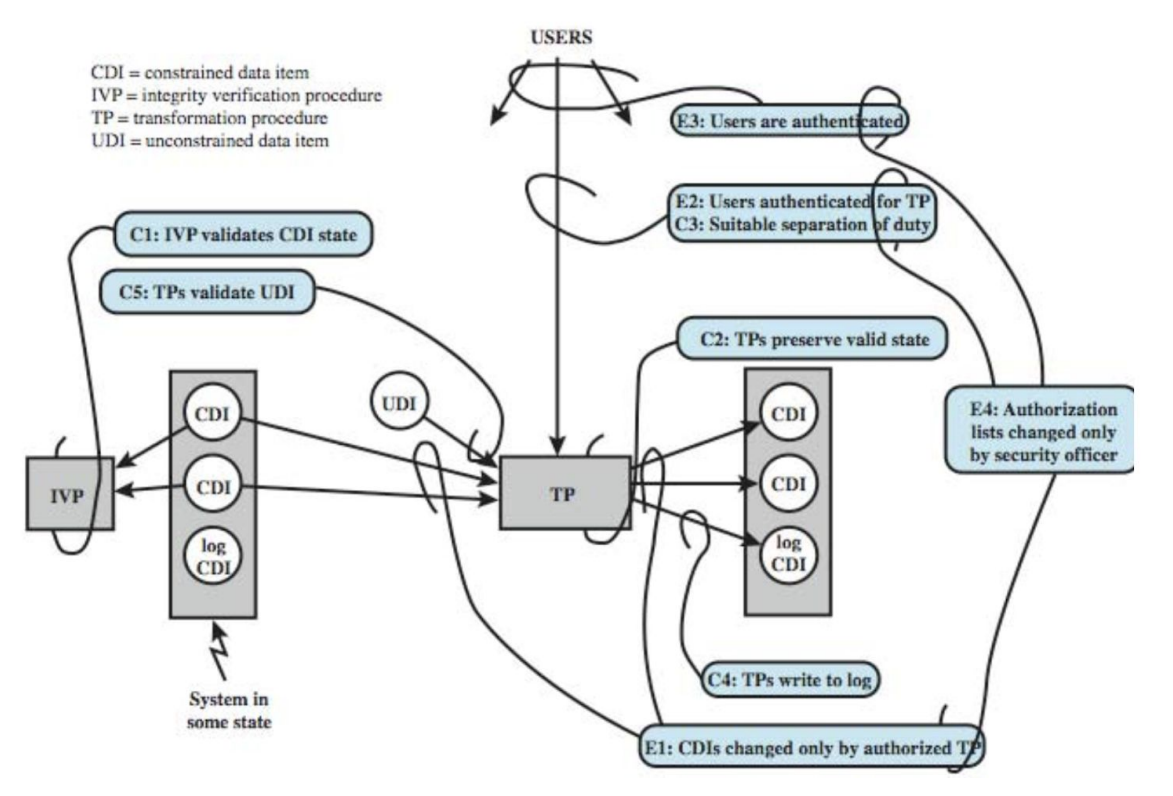
\includegraphics[width=10cm, keepaspectratio]{capitoli/policy/imgs/clark_wilson5.png}
\end{figure}

\subsubsection{I principali limiti}
\begin{itemize}
      \item Staticità delle relazioni di autorizzazione,
      \item Staticità della separazione dei compiti,
      \item Concessione centralizzata delle autorizzazioni assegnata all'
            amministratore della sicurezza.
\end{itemize}

\subsubsection{Biba vs. Clark-Wilson}
In Biba la fiducia nei soggetti viene valutata in base alle azioni
che soddisfano le regole e non in base alla nozione di regola di certificazione.
I dati non fidati
vengono esaminati prima di essere dichiarati fidati. In Clark-Wilson ci sono
degli espliciti requisiti
che regolano le azioni che possono essere fatte; inoltre le entità fidate devono
certificare il metodo
per aggiornare il dato da non fidato a fidato (e non il dato stesso).
Biba si basa sull'integrità multi-livello, mentre Clark-Wilson focalizza la
separazione dei compiti e
delle transazioni.